\chapter{The graph-based tool}

% INTRODUCTION %

In this chapter we describe the tool that we have developed to perform analysis and populating of pre-generated maps using \<Graph Theory>. After a quick overview, we introduce the analysis capabilities of this tool and then we present how we have employed them, together with Graph Theory, to strategically place resources in pre-generated maps.

% DESCRIPTION %

\section{Description of the tool}

This tool generates different kind of graphs, starting from the text and the All-Black representation of a map, that are used to perform various analysis and manipulation operations.

\par

The use of All-Black format is convenient, because it provides by default a logical division of the map in different areas and it allows our tool to be applied by other researchers, since as we have seen the All-Black format is widely used in this field. We have used this tool to position resources in a pre-generated map, but, for instance, it could be used to address the identification and definition of design patterns from an unfamiliar perspective or for \<direct evaluation> in Search Based PCG.

\par 

We developed this tool in \<Python> because if offers many solid Graph Theory libraries, as \<NetworkX>, that is the one we have used.

% ANALYSIS %

\section{Analysis of pre-generated maps}

The analysis is performed by generating different kind of graphs, each one used to highlight a different feature of the map in question.

\subsection{Outlines graph}

The \<outlines graph> is generated starting from the All-Black representation of a map and is obtained by associating a node to every vertex of every room and corridor and by connecting the non-adjacent ones that belong of the same outline. This graph has a single kind of node (\<vertex node>), which contains the coordinates of the tile it represents, which are used to position the node when the graph is visualized. Figure \ref{img:graph_out} shows an example of this graph.

\par

This graph can be used to visualize the rooms which compose the map.

\subsection{Reachability graphs}

Our tool can generate various kinds of \<reachability graphs> that represent various ways in which an entity can navigate a map. In these graphs a \<node> represents a position that an entity can reach, whereas an \<edge> indicates a viable path from a position to another.

\subsubsection{Tiles graph}

The \<tiles graph> is generated starting from the text representation of a map and is obtained by associating a node to each empty tile and by connecting each node to its corresponding 8-neighbors. The horizontal and vertical edges have cost $1$, whereas the diagonal ones have cost $\sqrt{2}$. This graph has a single kind of node (\<tile node>), which contains the coordinates of the tile it represents, which are used to position the node when the graph is visualized. Figure \ref{img:graph_tile} shows an example of this graph.

\par

This graph can be used to find the minimum distance that separates two cells, along with the shortest path that connects them.

\subsubsection{Rooms graph}

The \<rooms graph> is generated starting from the All-Black representation of a map and is obtained by associating a node to each room and corridor and by connecting nodes which corresponding rooms or corridors overlap with each other, using as weight the Euclidean distance of their central tile. This graph has a single kind of node (\<room node>), used to represent both rooms and corridors, which contains the coordinates of the closest and furthest vertex of the room from the origin. When visualized, each node is positioned on the coordinates of the central tile of the room it represents. Figure \ref{img:graph_room} shows an example of this graph.

\par

This graph can be used to analyze the topology of a map, in order to find loops, choke points, central areas and other kind of rooms.

\subsubsection{Rooms and resources graph}

The \<rooms and resources graph> is an extension of the room graph, which also include resources as nodes, that are connected to the nodes corresponding to the rooms and corridors which contain them. In addition to the room node inherited form the rooms graph, this graph has a node to represent resources (\<resource node>), which contains the coordinates of the resource, which are used to visualize the node, and the character associated to the resource. Figure \ref{img:graph_room_res} shows an example of this graph.

\subsection{Visibility graph}

The \<visibility graph> is generated starting from the text representation of a map and is obtained by associating a node to each empty tile and by connecting each node to all the tiles that are visible from that node. For two tiles to be respectively visible, it must be possible to connect them with a line without crossing any filled tile. This graph has a single kind of node (\<visibility node>), which contains the coordinates of the tile it represents, which are used to position the node when the graph is visualized, and its \<degree centrality>, i.e. the number of edges incident to that node. 

\par

To make this graph easier to read by the user, the tool associates a color to the nodes, which ranges from blue, for the one with the minimum visibility, to red, for the one with the maximum visibility. This can be seen in figure \ref{img:graph_visibility}.

\par

This graph can be used to analyze which areas of the map are more exposed and which ones are more repaired.

\begin{figure}[]
	\centering
  	\begin{subfigure}[t]{0.45\linewidth}
		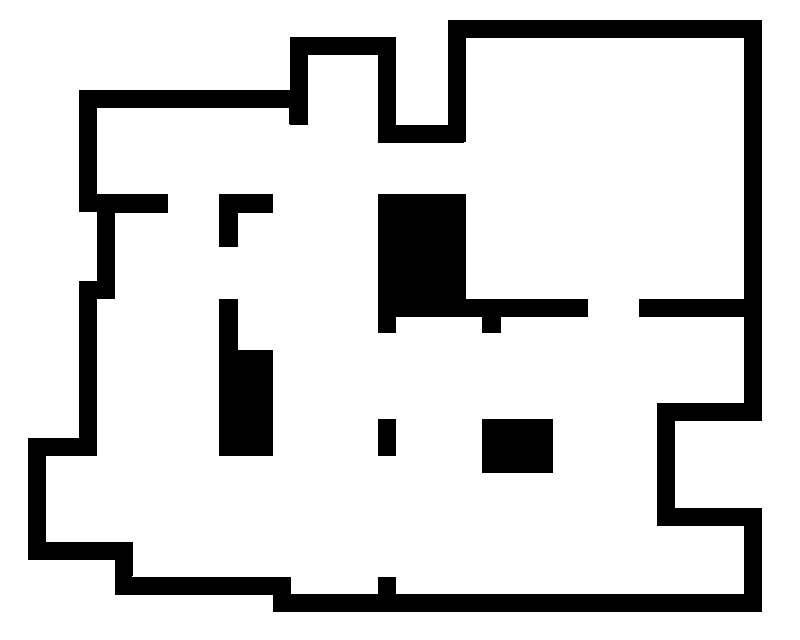
\includegraphics[width=\linewidth]{graph_divisive}
     		\caption{The map.}
     		\label{img:graph_divisive}
 	\end{subfigure}
  	\begin{subfigure}[t]{0.45\linewidth}
    		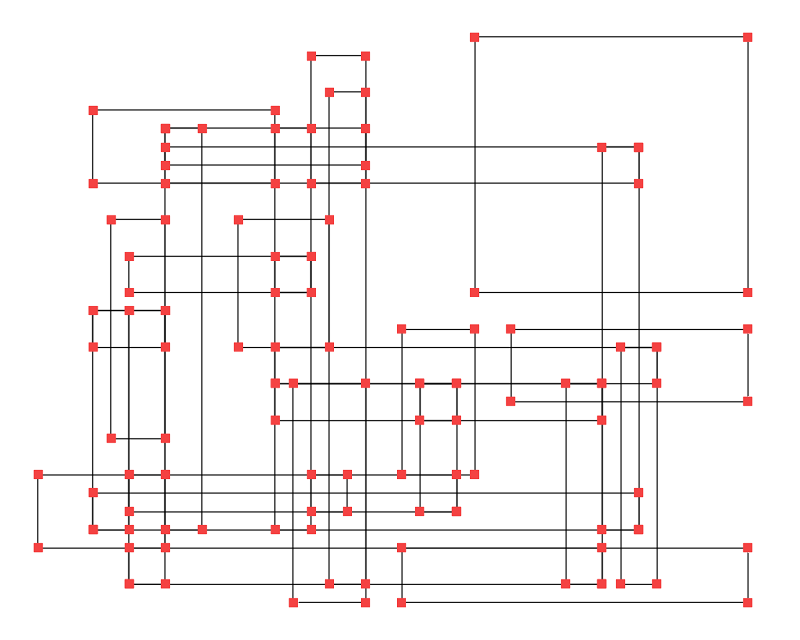
\includegraphics[width=\linewidth]{graph_out}
    		\caption{The outlines graph of the map.}
     		\label{img:graph_out}
  	\end{subfigure}
  	\begin{subfigure}[t]{0.45\linewidth}
    		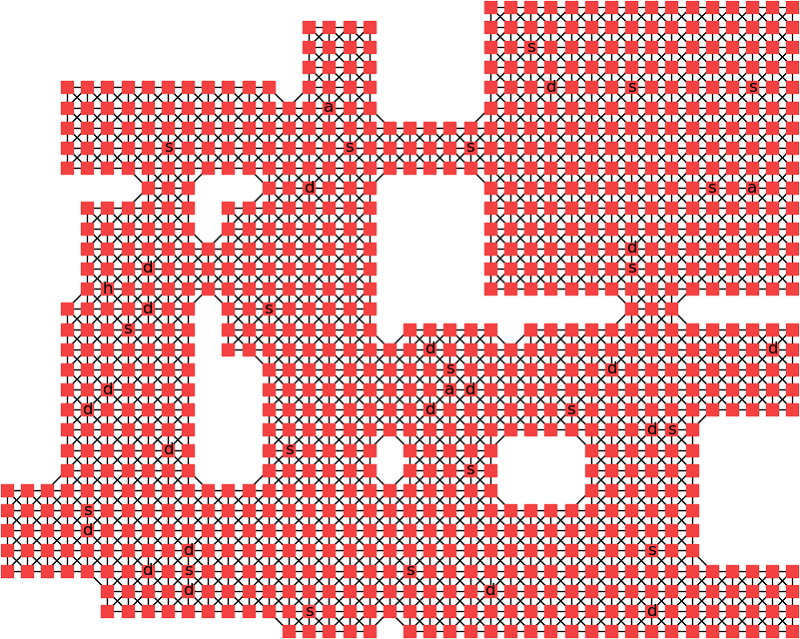
\includegraphics[width=\linewidth]{graph_tile}
    		\caption{The tiles graph of the map.}
     		\label{img:graph_tile}
  	\end{subfigure}
  	\begin{subfigure}[t]{0.45\linewidth}
    		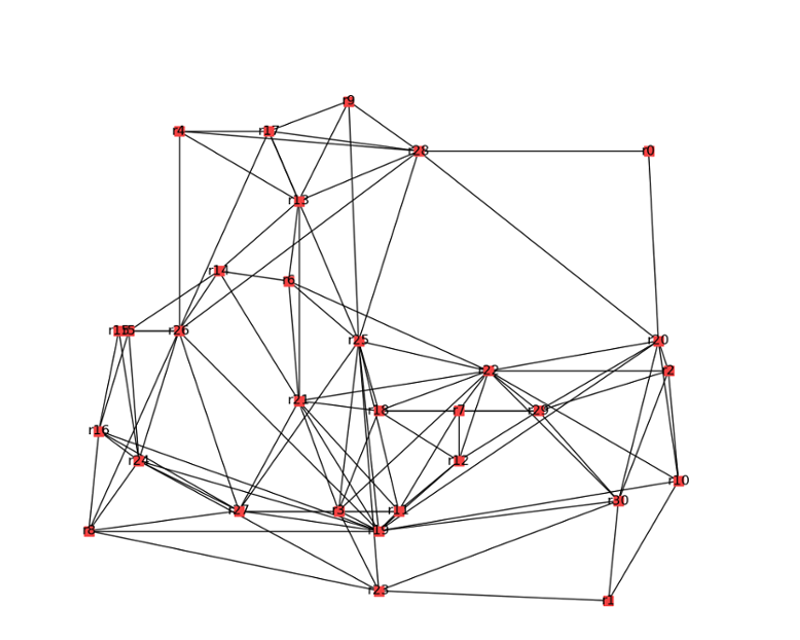
\includegraphics[width=\linewidth]{graph_room}
    		\caption{The rooms graph of the map.}
     		\label{img:graph_room}
 	\end{subfigure}
  	\begin{subfigure}[t]{0.45\linewidth}
    		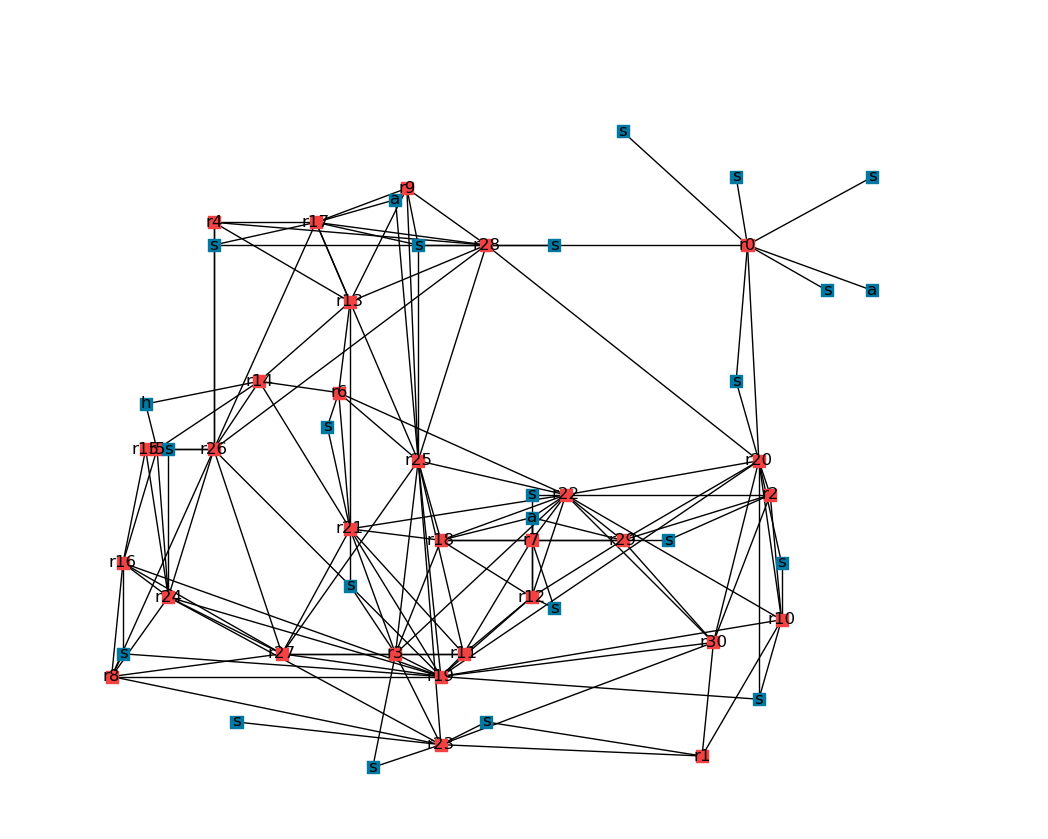
\includegraphics[width=\linewidth]{graph_room_res}
    		\caption{The rooms and resources graph of the map.}
     		\label{img:graph_room_res}
  	\end{subfigure}
  	\begin{subfigure}[t]{0.45\linewidth}
    		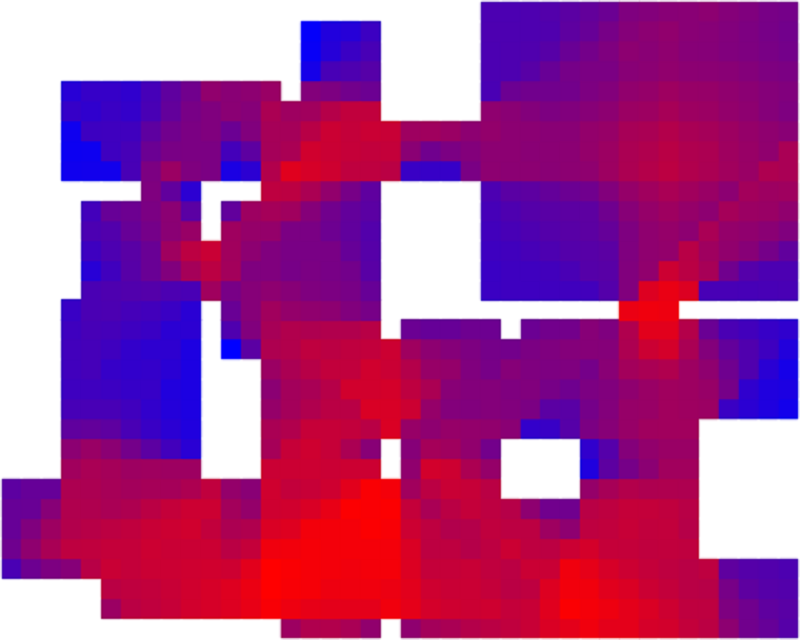
\includegraphics[width=\linewidth]{graph_visibility}
    		\caption{The visibility graph of the map.}
     		\label{img:graph_visibility}
  	\end{subfigure}	
	\caption{A map and all the graphs that the tool can generate from it.}
\end{figure}

\subsection{Interesting metrics}

Considering the graphs, in particular the ones with rooms and corridors as nodes, the following metrics defined by Graph Theory provide interesting information about the layout of a map:

\begin{itemize}
\item \<Degree centrality>: defined for a node, it is the number of edges that the node has. If the node represents a room, it measures how many entrance or exits the room has.
\item \<Normalized degree centrality>: defined for a node, it is obtained by normalizing the degree centrality, associating 0 to the node with the minimum centrality and 1 to the node with the maximum centrality.
\item \<Closeness centrality>: defined for a node, it measures its centrality in the graph, computed as the sum of the lengths of the shortest paths between the node and all other nodes in the graph. If the node represents a room, it measures how central the room is.
\item \<Betweenness centrality>: defined for a node, it measures its centrality in the graph, computed as the number of shortest paths connecting the nodes in the graph that pass through the node. If the node represents a room, it measures how central the room is.
\item \<Connectivity>: defined for a graph, it is the minimum number of elements (nodes or edges) that need to be removed to disconnect the remaining nodes from each other. If the graph represents a map, it measures the existence of isolated areas.
\item \<Eccentricity>: defined for a node, it is the maximum distance from the node to all other nodes in the graph. If the node represents a room, it measured how isolated the room is.
\item \<Diameter>: defined for a graph, it is the maximum eccentricity of its nodes. If the graph represents a map, it measures the size of the map.
\item \<Radius>: defined for a graph, it is the minimum eccentricity of its nodes. If the graph represents a map, it measures how distanced the rooms are from each other.
\item \<Periphery>: defined for a graph, it is the set of nodes with eccentricity equal to the diameter. If the graph represents a map, it defines its peripheral areas.
\item \<Center>: defined for a graph, it is the set of nodes with eccentricity equal to the radius. If the graph represents a map, it defines its central areas.
\item \<Density>: defined for a graph, it ranges from 0 to 1, going from a graph without edges to a complete graph. If the graph represents a map, it measures how complex it is.
\end{itemize}

% POPULATING %

\section{Populating of pre-generated maps}

We have defined multiple heuristics to populate a map with spawn points and resources using the metrics that can be extracted from a graph. These heuristic are a mathematical transposition of rules and patterns concerning resource placement that we have extracted from the work of Tim Schäfer\cite{great1vs1}, who has performed an in depth analysis of multiplayer 1vs1 maps for \<Quake 2>\footnote{Id Software, 1997}.


\subsection{FPS map analysis}

The balance of a deathmatch game radically changes each time that a player is killed. If the game has more than two players, the player who won the fight does not gain any strategic advantage, since he still has the other players to face, whereas the defeated player is put at considerable disadvantage, because on death he loses all the weapons and ammunition that he collected. In a 1vs1 match, a kill has an even stronger influence, since the surviving player has more weapons and ammunition and gains the complete control of the map, that comes with the chance of scoring another easy kill, as soon as the other player respawns, or of searching for additional equipment. Schäfer refers to the surviving player as \[up-player] and to the defeated one as \[down-player].

\par

To obtain a multiplayer map that is interesting and fun to play it is important to consider the up-player vs down-player dynamic both when defining the map layout and when positioning resources.

\par

The spawn points, i.e. the locations where the down-player reappears, should be positioned in areas that are of low interest for the up-player and that are easy to leave. Obviously, central hubs and dead ends are a bad choice, whereas rooms with 2 or 3 exits are usually the best option. 

\par

For what concerns the resources, they must be placed considering both the up-player vs down-player dynamic and the characteristics of the resource itself. It is important to place the right amount of resources on the map, because too many would eliminate the need for exploration, whereas too few would further disadvantage the down player. It is also important not to place too many powerful items in the same area or in boring spots, since the risk to obtain them should always be proportional to the strategical advantage they allow to achieve. It is important to consider that a powerful resource is interesting for both players, so it often acts as a \<point of collision>. The resources usually are of five kinds: health pack, armor, power-up, ammunition and weapon. 

\par

The health packs are placed in zones that are safe or not too dangerous. They have no use for the down-player, that respawns with full health, but they can be useful for the up-player, if he has been damaged during the fight, whereas they always come in handy during a fight or when one of the contenders disengages.

\par

Armor, which is a second health that is consumed before the main one, is usually placed in spots that are aimed both at the down-player and at the up-player: objects that provide a small quantity of armor should be easy to achieve, whereas the ones that provide full armor should be placed in dangerous areas.

\par

Power-ups grant temporary advantages to the player who collects them, like invisibility or increased damage, and are placed in locations difficult to reach. 

\par 

The position of a weapon and of its ammunition depends on the weapon itself. We can divide the weapons in three categories: weak, medium and strong. Weak weapons are of a certain interest for the down-player, if he has not collected any other weapon yet, and of no interest for the up-player, so they are placed near spawn-points or in gaps where no other weapon is available, together with their ammunition. Medium weapons are of high interest for the down-player, since he needs to get one of them as soon as possible if he wants to face the up-player, so they are placed in areas that are easy to reach and the same goes for their ammunition. Finally, the strong weapons should be placed in areas that are strategically disadvantageous, like dead ends or vertically dominated areas, or difficult to reach. If a weapon is very contextual, i.e. it is useful in very few situations, it is usually placed in an area that allows to take advantage of its features, whereas a weapon that is strong in almost any situation is usually placed in an area where it cannot be used optimally (e.g. a rocket launcher in a small room).

\subsection{Spawn points placement}

We have defined four heuristics for the placement of spawn points. 

\subsubsection{Low risk heuristic}

This method selects rooms that have a low number of entrances, are not dead ends and are distant from each other and for each one of them places the spawn point on the tile that offers the best balance between low visibility and distance from the walls. In this way spawn points are placed in passageways that are sheltered and easy to leave. 

\par

Given $G$ the rooms and corridors graph, $R \subset G$ the subset of room nodes, $S \subset G$ the subset of resource nodes (that in this case is composed exclusively by the already positioned spawn points) and $n$ the total number of spawn points that must be added to the map, the most suitable room for containing  a spawn point is selected with the following heuristic:

\begin{align*}
 &  room = \argmax_{r \in R}\vast(  w_2 \times \min_{n \in G}
  	\begin{cases}
    		\hfil 1 & \text{if } n \in S \\
    		\cfrac{\spl(r, n)}{\diam(G)} & \text{if } n \in S \
  	\end{cases} \vast\} \\ 
  	 & + w_1 \times
	\begin{cases}
    		\hfil 0 & \text{if } \degcent(s) = 1 \\
    		1 - \cfrac{\degcent(r) - \min_{r' \in R}\degcent(r')}{\max_{r' \in R}\degcent(r') - \min_{r' \in R}\degcent(r')} & \text{if } \degcent(r) \neq 1 \
  	\end{cases} \vast\}
	\vast)
\end{align*}

The first component of the equation, which is weighted by $w_2$, promotes rooms with few passages but that are not dead ends, whereas the second component, which is weighted by $w_1$, promotes rooms that are distant from the already placed spawn points. Both are normalized to the interval $[0,1]$ and their influence is proportional to their weights. We experimentally found that the values which provide the best results are $ w_1 = 1 $ and $ w_2 = 0.5 $.

\par

Once that the room has been found, one of its tiles is selected with the support of the visibility graph. Given G the visibility graph, $T \subset G$ the subset of nodes that belong to the room, $S \subset G$ the subset of nodes that contain resources (that in this case is composed exclusively by the already positioned spawn points), the most suitable tile for containing a spawn point is selected with the following heuristic:

\begin{align*}
tile = \argmax_{t \in T} & \vast( w_1 \times \vast( 
    		1 - \cfrac{\degcent(t) - \min_{t' \in G}\degcent(t')}{\max_{t' \in G}\degcent(t') - \min_{t' \in G}\degcent(t')} \vast) \\
  	 &\quad +  w_2 \times \cfrac{\walld(t, room)}{ \maxwalld(room)} \\
  	 &\quad  + w_3 \times
  	\begin{cases}
    		\hfil 0 & \text{if } | S | = 0 \\
    		\min_{s \in S}\cfrac{\cartd(t, s)}{d}& \text{if }  | S | > 0 \
  	\end{cases} \vast\}
	\vast)
\end{align*}

The first component of the equation, which is weighted by $w_1$, promotes tiles with low visibility, the second component, which is weighted by $w_2$, promotes tiles that are distant from the walls, whereas the third component, which is weighted by $w_3$, promotes tiles that are distant from already placed spawn points. All three components are normalized to the interval $[0,1]$ and their influence is proportional to their weights. We experimentally found that the values which provide the best results are $ w_1 = 1 $ and $ w_2 = 0.5 $ and $ w_3 = 0.5 $.

\subsubsection{Uniform heuristic}

This method selects rooms that are uniformly distributed in the map and for each one of them places the spawn point on the tile that offers the best balance between low visibility and distance from the walls. 

\par

The first room is selected at random, then, given $G$ the rooms and corridors graph, $R \subset G$ the subset of room nodes, $S \subset G$ the subset of resource nodes (that in this case is composed exclusively by the already positioned spawn points), the remaining rooms are selected with the following heuristic:

\begin{align*}
	room = \argmax_{r \in R} ( \min_{s \in S} (\spl(r, s) ))
\end{align*}

\par

Once that the room has been found, one of its tiles is selected using the low risk heuristic. 

\subsubsection{Random heuristic}

\subsection{Ammunition placement}

\subsection{Health packs placement}

% SUMMARY %

\section{Summary}